\documentclass[12pt]{article}

\usepackage{csquotes}
\usepackage[spanish]{babel}
\usepackage[hidelinks]{hyperref} % So the Table of Contents to has links to the sections
\usepackage{xcolor} % For the hyperref link colors
\usepackage[backend=biber, style=numeric, citestyle=numeric]{biblatex}
\usepackage{graphicx} % To embed images
\usepackage{cleveref} % To reference with cref and see the name of the object

\hypersetup{colorlinks = true, linkcolor={blue!50!black}, citecolor={blue}}
\addbibresource{Resources/Bibliography/bibliography.bib} % Imports bibliography file
\graphicspath{ {Resources/Images/} } % Sets the path to look for images 
\title{Base de datos y Hadoop}
\author{Carlos Domínguez García (alu0100966589@ull.edu.es)}
\date{17 de febrero de 2019}

\begin{document}

  \maketitle
  \pagebreak
  
  \tableofcontents
  \pagebreak

  \section{Introducción}
    Sin bases de datos la única manera de almacenar datos de manera persistente es interactuando con el sistema de almacenamiento. Esto que implica que las aplicaciones, para poder usar los datos tengan que implementar operaciones CRUD (Create, Read, Update, Delete) sobre el sistema de almacenamiento. Por ejemplo, es común interactuar a través de un sistema de archivos, en este caso las aplicaciones tienen que encargarse de abrir o crear los archivos, entender el formato del contenido, actualizar el contenido escribiendo en el fichero y cerrarlo.

    Esta añadida complejidad de las aplicaciones abre la posibilidad a una mayor cantidad errores en su código. Pero también, debido la falta de una manera estándar de acceder a los datos, cada aplicación podría implementar el manejo de los datos de manera distinta provocando redundancia si aplicaciones que necesitaban los mismos datos los almacenaban en distintos ficheros, inconsistencia si estos datos duplicados unos se actualizaban y otros no, etc. \cite{MariaDB_EarlyDatabaseModels}

    Para resolver esta situación surgieron los sistemas gestores de bases de datos. Este tipo de sistema se sitúa entre los usuarios y el sistema de almacenamiento, proporcionando una estructura lógica de los datos y una interfaz que permite a los usuarios referirse a los datos según la estructura lógica. De esta manera pueden usar una interfaz con un alto nivel de abstracción y no se tienen que preocupar de los problemas relacionados con interactuar directamente con los ficheros ya que el sistema también se encarga de ello.
    
    El primer modelo de datos fue el modelo jerárquico \cite{MariaDB_HierarchicalDatabaseModel}. Aquí los datos se disponen en una colección de valores llamados registros, que están relacionados por enlaces de nodos padres a hijos simulando una estructura de árbol invertido. Sin embargo, este modelo lleva consigo algunos inconvenientes como que no es bueno para representar relaciones muchos a muchos. Por ejemplo, alumnos inscritos a varias clases y clases con varios alumnos como se puede observar en \cref{fig:HierarchicalModelManyToMany}. Además, añadir nuevas relaciones puede implicar que se tenga que cambiar toda la estructura. Por último, para referirse a un dato los usuarios han de conocer bien la estructura para saber qué enlaces recorrer.

    \begin{figure}[h]
      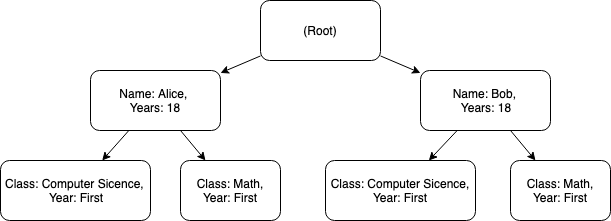
\includegraphics[width=\textwidth]{HierarchicalModelManyToMany.png}
      \centering
      \caption[Representación de una relación muchos a muchos en el modelo jerárquico]{Representación de la relación muchos a muchos en el modelo jerárquico, en concreto se puede observar que para cada alumno de primer año se han de repetir los registros de las asignaturas}
      \label{fig:HierarchicalModelManyToMany}
    \end{figure}

  \section{Base de datos relacionales}
    TODO:
    Relational model, ACID, normalization... scaling (vertical, horizontal for read and writing)
  
  \section{Base de datos distribuidas}
    TODO:
    Scalability (horizontal, vertical), CAP, problems with ACID. big data... and thats why nosql

    - https://www.infoq.com/articles/cap-twelve-years-later-how-the-rules-have-changed

  \section{Base de datos NoSQL (Not only SQL)}
    TODO:
    Mongo, Cassandra, HBase(?). Where each fits in CAP

    - https://www.3pillarglobal.com/insights/short-history-databases-rdbms-nosql-beyond
    - https://stackoverflow.com/questions/48240702/mongo-and-cassandra-in-context-of-cap
    - https://www.scnsoft.com/blog/cassandra-vs-hadoop

  \section{Hadoop}
    TODO:
    nosql vs hadoop (NoSQL use cases often entail end user interactivity, like in web applications, but more broadly they are about reading and writing data very quickly. Hadoop, on the other hand, is about large-scale processing of data. To process large volumes of data, you want to do the work in parallel, and typically across many servers. -- https://mapr.com/blog/hadoop-vs-nosql-whiteboard-walkthrough/)
    \subsection{HDFS}
    \subsection{MapReduce}
    \subsection{YARN}

  \section{Spark}
    TODO:
    Batch processing vs Stream processing

    - https://medium.com/stream-processing/right-tool-for-the-job-why-you-shouldnt-do-stream-processing-with-mapreduce-539e180565e6
    - https://medium.com/@gowthamy/big-data-battle-batch-processing-vs-stream-processing-5d94600d8103
    - https://www.quora.com/What-is-stream-processing-in-big-data-and-what-does-it-do

  
  \printbibliography
  
\end{document}